\begin{tikzpicture}[font=\bf\sffamily\fontsize{9}{9}\selectfont]


  
  \def\COLH1N1{Red1}
  \def\COLBx{Red4}
  \def\COLCx{Green1}
    \def\COLDx{Green4}
    \def\COLEx{Blue1}

   
\node[] (A) at (0,0) {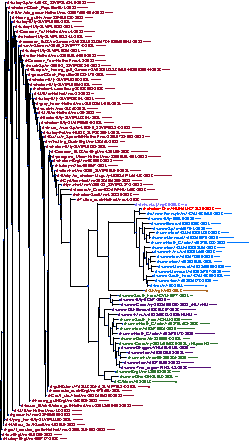
\includegraphics[width=.9\textwidth]{Figures/riskyphylo625_collapsed_20}};

 \draw[line width=2pt] ([yshift=8.75in,xshift=1.75in]A.south) node[label={[]-90: $\bigstar$: sequences withg CDC-IRAT scores}] (DA) [left,below]{6.0} -- ++(.65in,0) node (DB) [right,below] {8.0};

 \node[anchor=south] (Lx1)  at ([xshift=.3in,yshift=.1in]DA.north) {estimated emergence score};
\coordinate (C1) at ([xshift=-.0in,yshift=0.1in]Lx1.north) ;
 \node[align=center,fill=colh1n1x,text=white,,text width=.35in,anchor=south,xshift=0in,yshift=0.02in,] (X1) at (C1.north) {H1N1};
 \node[align=center,fill=colh1n2x,text=white,,text width=.35in,anchor=south,xshift=0in,yshift=0.02in,] (X1) at (X1.north) {H1N2};
 \node[align=center,fill=colh3n2x,text=white,,text width=.35in,anchor=south,xshift=0in,yshift=0.02in,] (X1) at (X1.north) {H3N2};
 \node[align=center,fill=colh5n1x,text=white,,text width=.35in,anchor=south,xshift=0in,yshift=0.02in,] (X1) at (X1.north) {H5N1};
 \node[align=center,fill=colh7n9x,text=white,,text width=.35in,anchor=south,xshift=0in,yshift=0.02in,] (X1) at (X1.north) {H7N9};
 \node[align=center,fill=colh9n2x,text=white,,text width=.35in,anchor=south,xshift=0in,yshift=0.02in,] (X1) at (X1.north) {H9N2};
 \node[align=center,fill=colh3n3x,text=white,,text width=.35in,anchor=south,xshift=0in,yshift=0.02in,] (X1) at (X1.north) {H3N3};

  \node[anchor=south] (Lx2)  at ([xshift=0in,yshift=.05in]X1.north) {subtype key};


\coordinate (L1) at ([xshift=-1.5in,yshift=.8in]A.south east) ;
\def\FCOLX{Red1}
\node[shape=isosceles triangle,fill=\FCOLX,rotate=-90,label={[yshift=.4in]0:7.73} ] (h1n1strain) at ([xshift=1.2in,yshift=4.35in]L1.north) {};
\node[shape=isosceles triangle,fill=\FCOLX,rotate=-90,label={[xshift=.05in,yshift=.4in]0:7.74}  ] (h1n1strain) at ([xshift=.5in,yshift=1.27in]L1.north) {};
\node[shape=isosceles triangle,fill=\FCOLX,rotate=180,label={[xshift=.55in,yshift=.01in]0:7.72} ] (h1n1strain) at ([xshift=-.15in,yshift=.735in]L1.north) {};
\node[shape=isosceles triangle,fill=\FCOLX,rotate=180 ,label={[xshift=.55in]0:7.41} ] (h1n1strain) at ([xshift=-.185in,yshift=5.845in]L1.north) {};
\node[shape=isosceles triangle,fill=\FCOLX,rotate=180,label={[xshift=.55in]0:7.42} ] (h1n1strain) at ([xshift=-.85in,yshift=6.44in]L1.north) {};
\node[shape=isosceles triangle,fill=\FCOLX,rotate=180,label={[xshift=.55in]0:7.73} ] (h1n1strain) at ([xshift=.7in,yshift=3in]L1.north) {};
\node[shape=isosceles triangle,fill=\FCOLX,rotate=180,label={[xshift=.55in]0:7.73} ] (h1n1strain) at ([xshift=.8in,yshift=3.15in]L1.north) {};

% \node[anchor=west] at ([xshift=.1in,yshift=-.1in]h1n1strain.east) {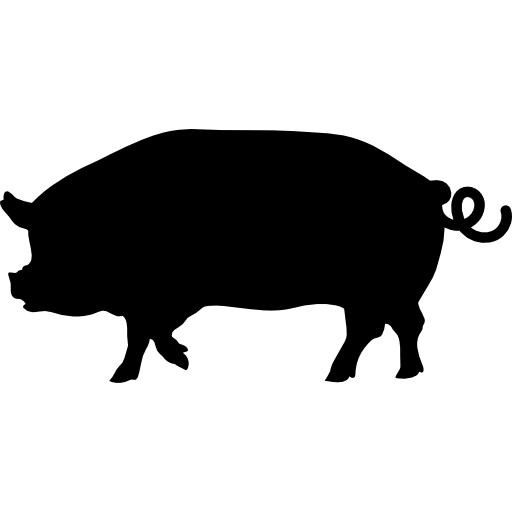
\includegraphics[width=.5in]{Figures/animalicons/pig}};

% \node[shape=isosceles triangle,fill=\FCOLX,rotate=-90 ] (h7n9strain) at ([xshift=.850in,yshift=4.65in]L1.north) {};
% \node[anchor=west] at ([xshift=-.2in,yshift=0.45in]h7n9strain.east) {
\includegraphics[width=.6in]{Figures/animalicons/camel}};

% \node[shape=isosceles triangle,fill=\FCOLX,rotate=-90 ] (h3n2strain) at ([xshift=1.22in,yshift=4.1in]L1.north) {};

 \node[anchor=west] at ([xshift=.2in,yshift=2.35in]L1.north) {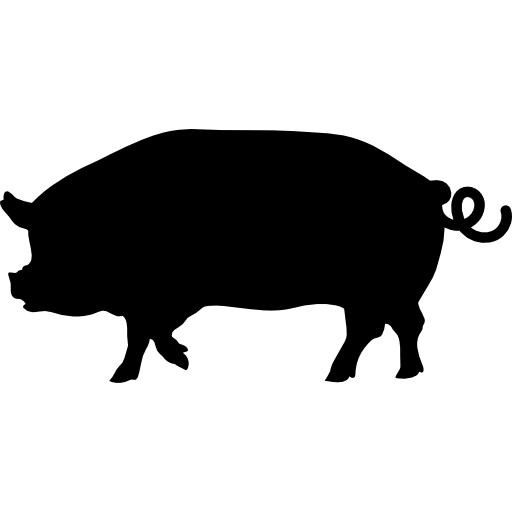
\includegraphics[width=.6in]{Figures/animalicons/pig}};

% \node[shape=isosceles triangle,fill=\FCOLX,rotate=-90 ] (h9n2strain) at ([xshift=.3in,yshift=4.8in]L1.north) {};
% \node[anchor=west] (mink) at ([xshift=-.265in,yshift=0.35in]h9n2strain.east) {
\includegraphics[width=.6in]{Figures/animalicons/mink}};
 \node[anchor=west] at ([xshift=-.5in,yshift=6.75in]L1.north) {\includegraphics[width=1in]{Figures/buzzard}};

 \node[anchor=west] at ([xshift=.2in,yshift=6in]L1.north) {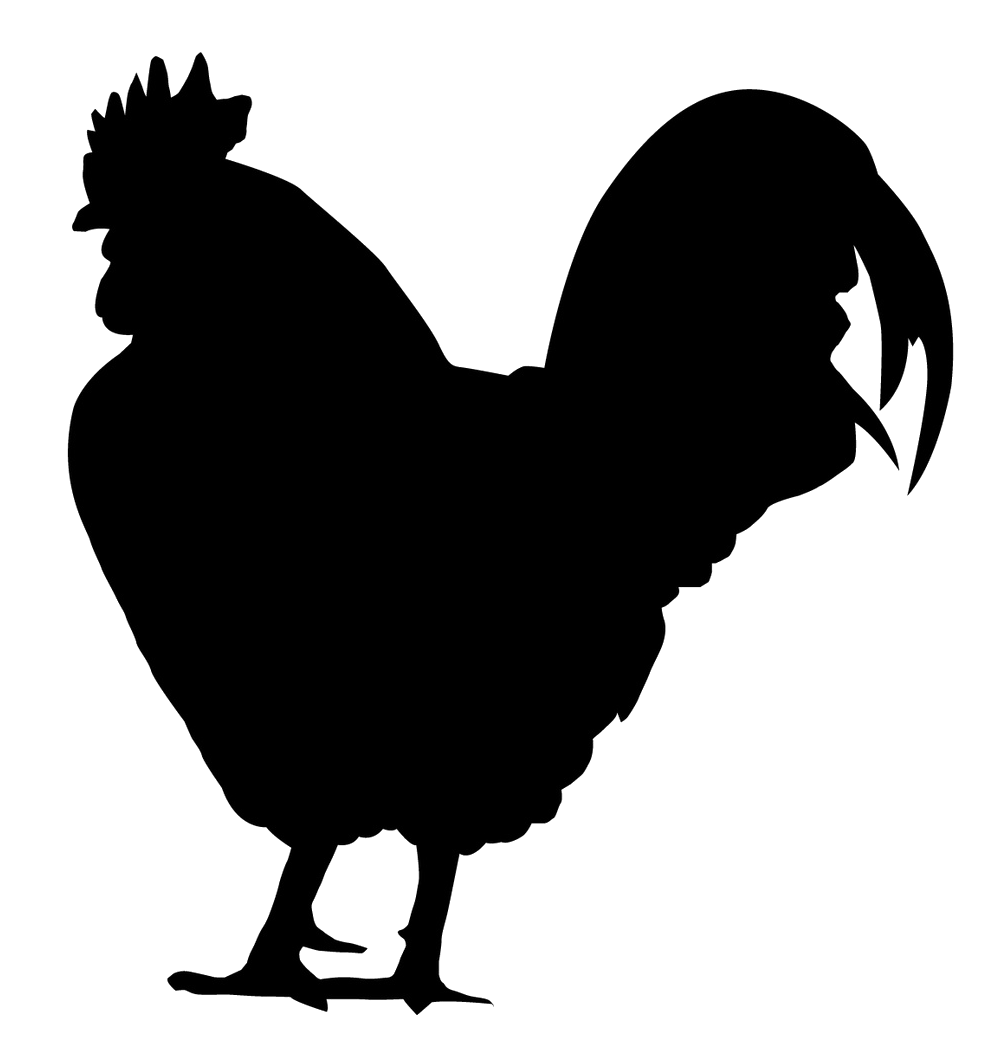
\includegraphics[width=.5in]{Figures/animalicons/chicken}};
% \node[anchor=west,opacity=.5] (dd) at ([xshift=-2.5in,yshift=-1.45in]h9n2strain.east) {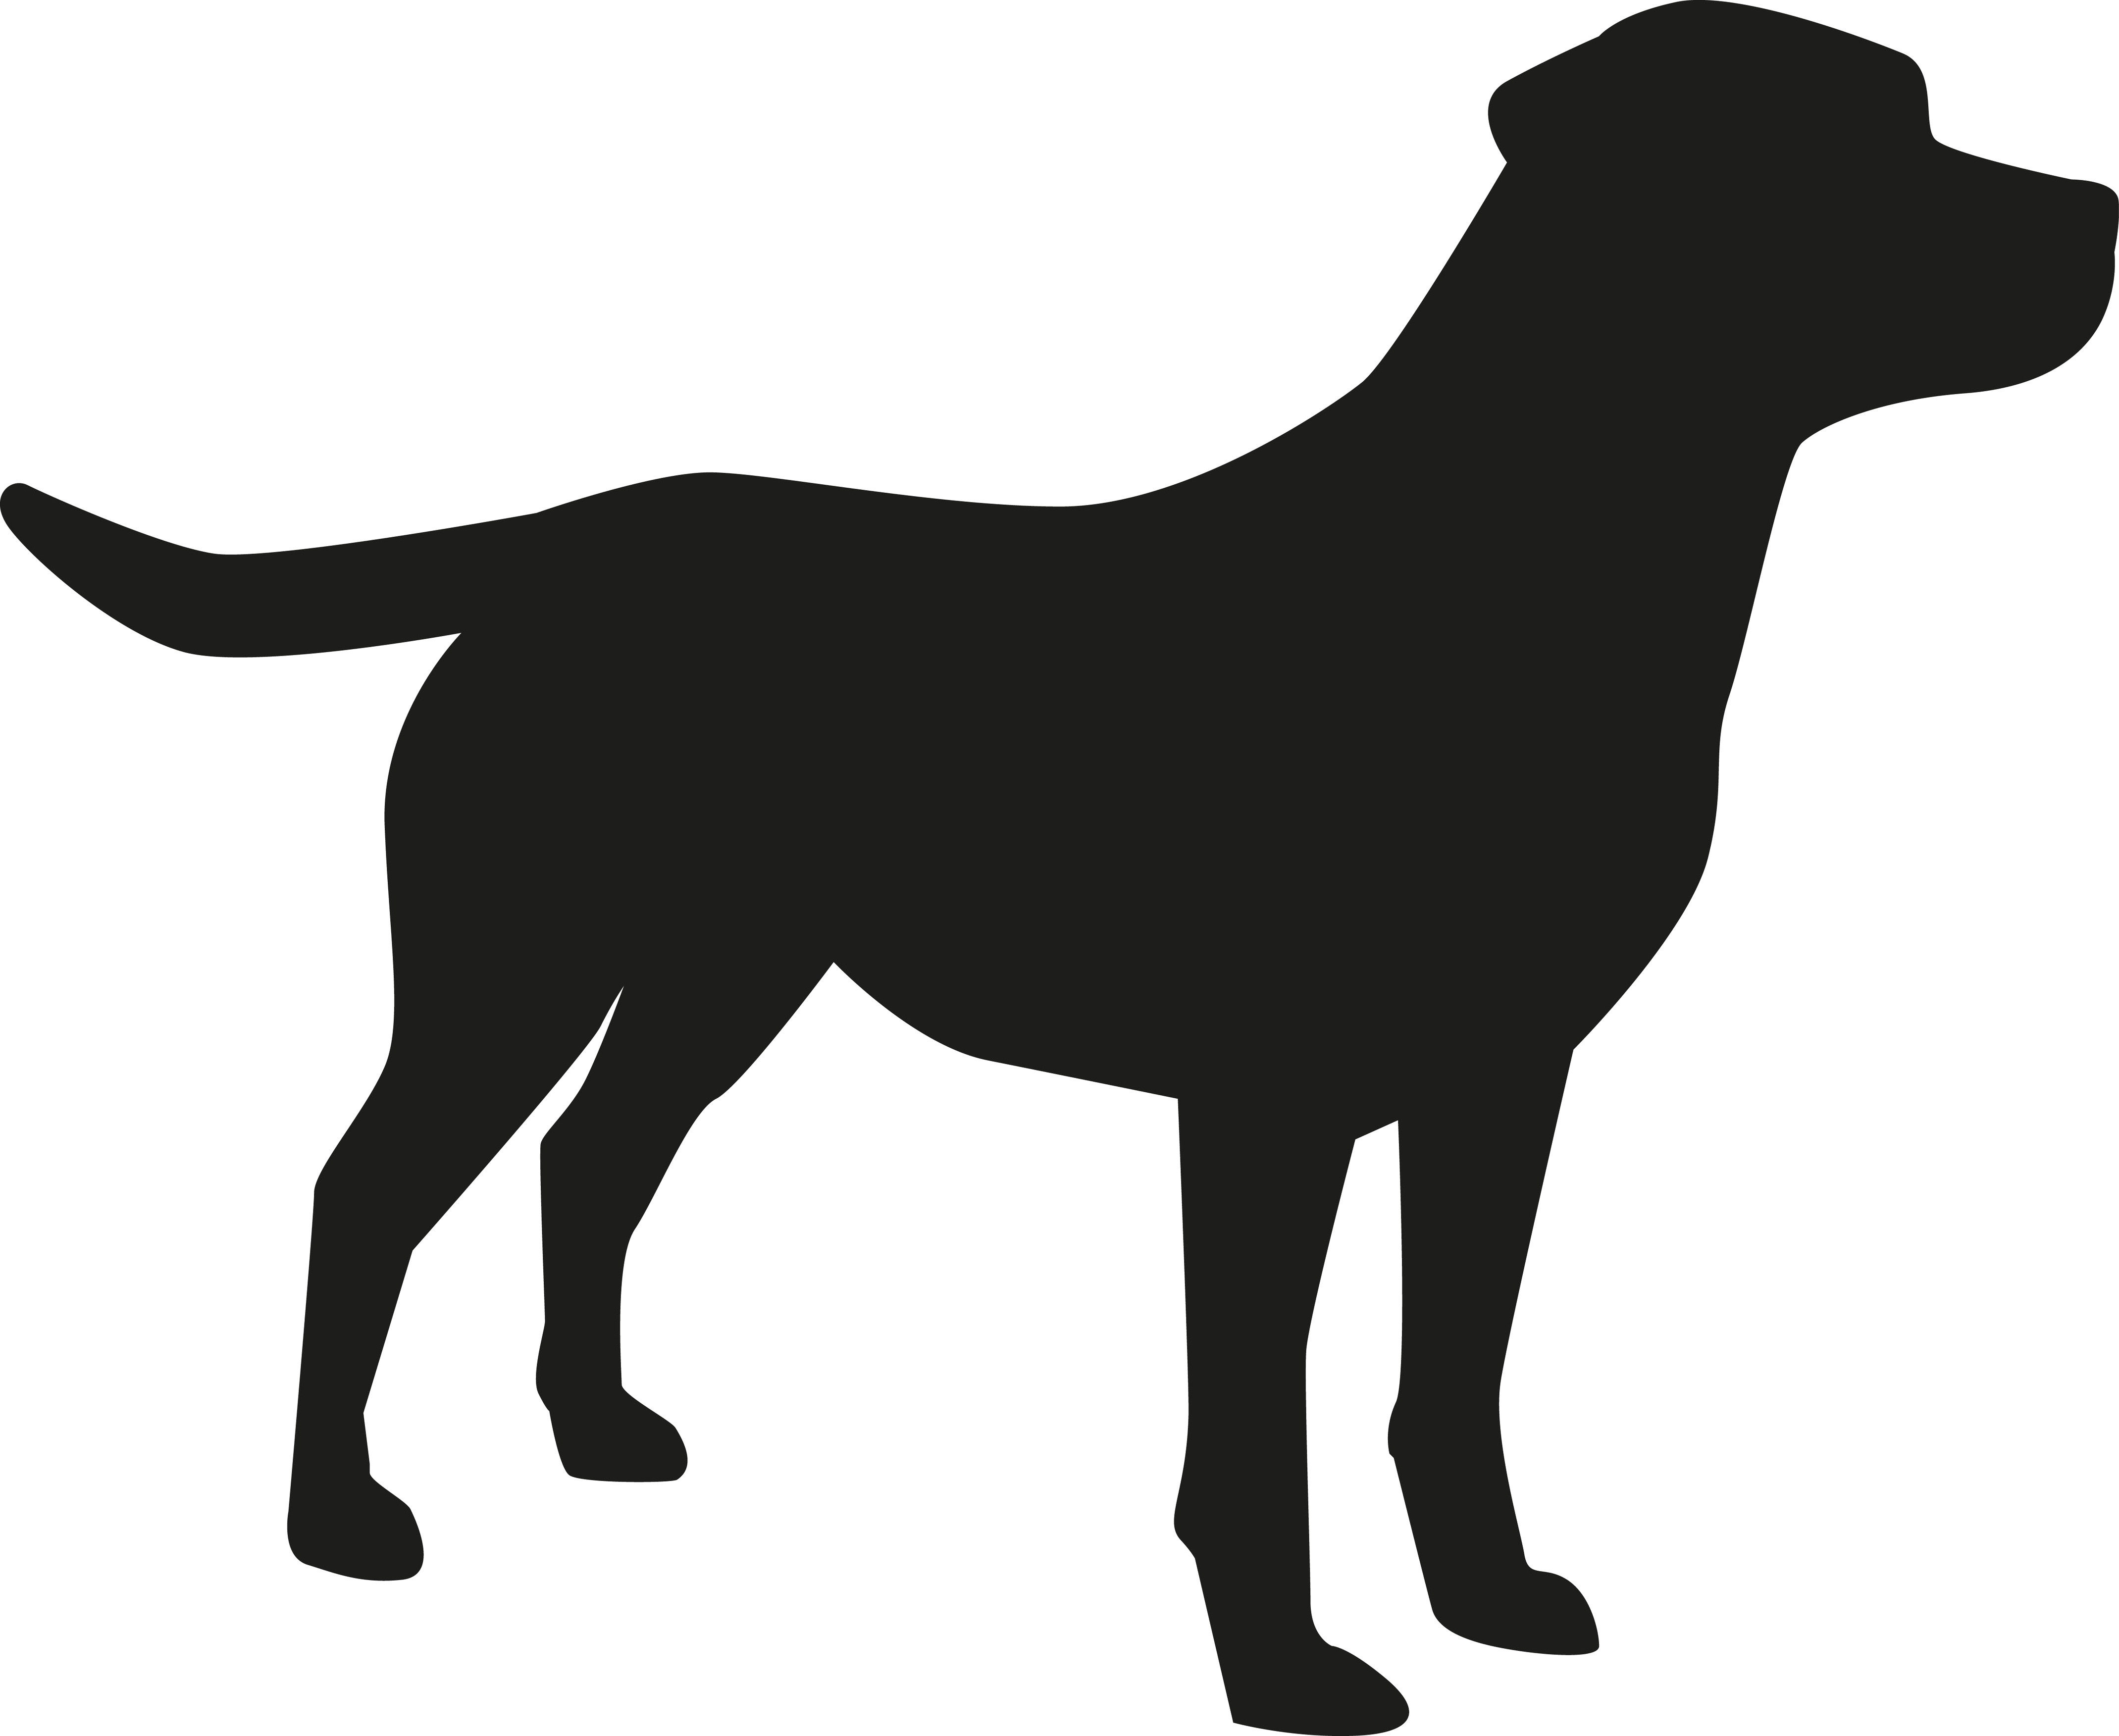
\includegraphics[width=.6in]{Figures/animalicons/dog}};
% \node[anchor=west,opacity=.5] (dc) at ([xshift=-2in,yshift=-1.85in]h9n2strain.east) {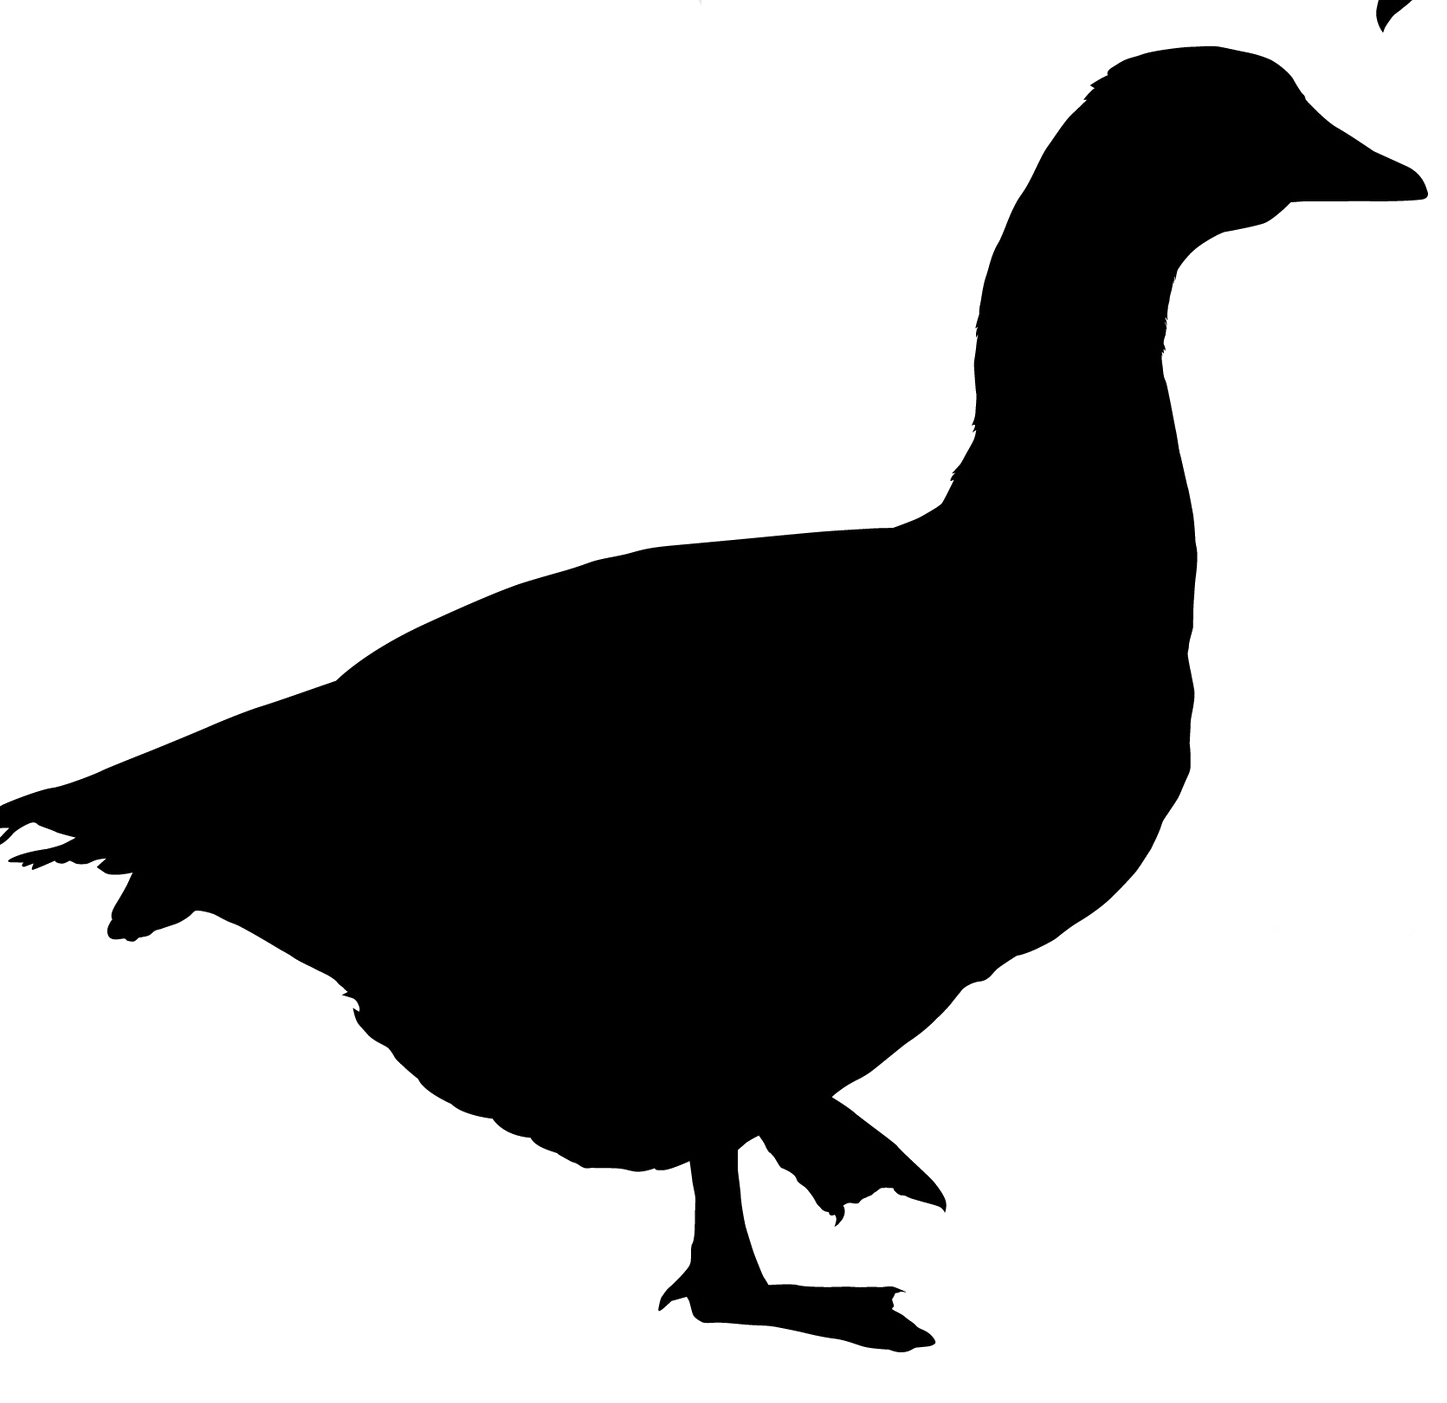
\includegraphics[width=.5in]{Figures/animalicons/duck2}};

% \node[anchor=south,opacity=.4] (pig2) at ([xshift=-2.2in,yshift=-5.5in]mink.north) {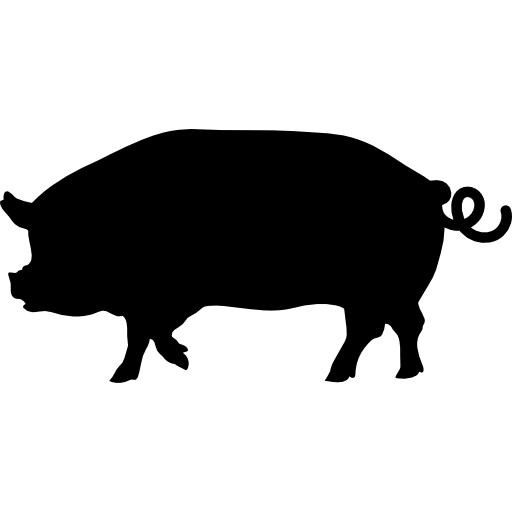
\includegraphics[width=.8in]{Figures/animalicons/pig}};

% \node[anchor=south,opacity=.4] (pig3) at ([xshift=-1in,yshift=1in]mink.north) {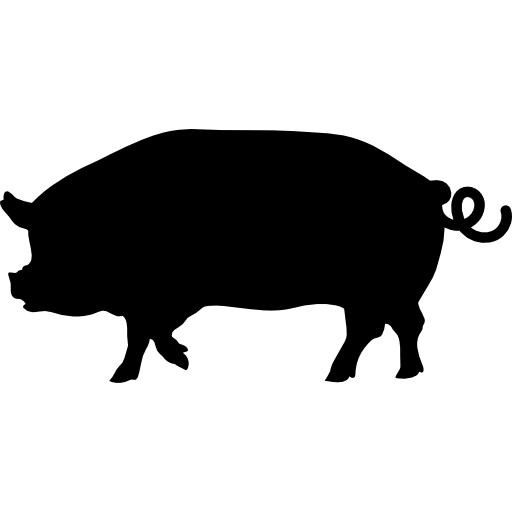
\includegraphics[width=.8in]{Figures/animalicons/pig}};


% \draw [ultra thick,dashed,opacity=.3] (cc) -- ++(1.1in,1in);
% \draw [ultra thick,dashed,opacity=.3] (dd) -- ++(.96in,1in);
% \draw [ultra thick,dashed,opacity=.3] (dc) -- ++(.55in,1.3in);

\end{tikzpicture}